\chapter{Results}

Figure \ref{fig:rel-error-100000} shows the accumulated absolute value of the relative, $|\varepsilon_{rel}|$, error for 100 000 highscore uppdates. The motivation for showing the accumulated error rather than just the relative error is that the plot of the accumulated relative error unveils the characteristics of the algorithms behaviours.

Note that while the slope for the solid line is positive, it is not to a measurable extent increasing for a test run of 100 000 rank estimates, ie. $|\varepsilon_{rel}|$ is practically constant.

\todo{Put legend in figure}

\begin{figure}[h!]
  \centering
  \caption{Accumulated relative error after 100 000 highscore updates. The dashed line is the original algorithm, the solid line is the improved algorithm.}
  \label{fig:rel-error-100000}
  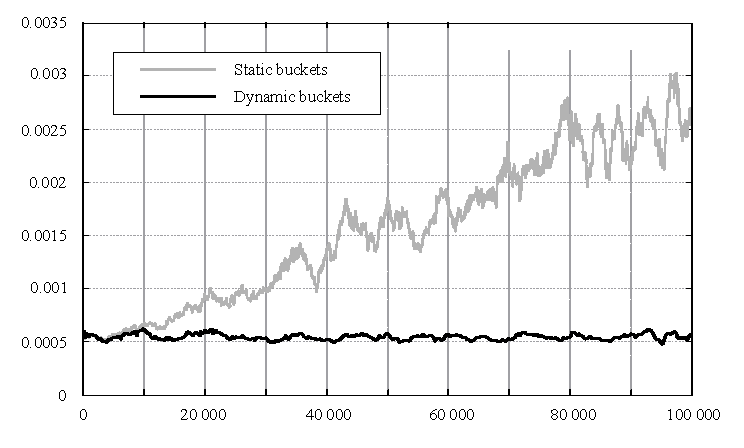
\includegraphics[width=12cm]{img/rel-error-100000.eps}
\end{figure} 

The hypothesis imply that the experiment should be done in three steps; one to find the size of the maximum error with the current configuration. That would be after 4000 highscore updates. The current algorithm have an average relative error in the range 3900 to 4099 is 0.00052\footnote{0.000517098}. 


and a second step measuring how much longer the new algorithm can run before reaching the same error levels. Finally, third step would be comparing the cost of the two approaches. 


The problem is defining the baseline error with the current implementation which creates a fresh bucket-table every 10 minutes (that is roughly every 4000 rankings). In the experiment, mean relative error in the range 1-1000 is actually larger than 3000-4000 with the current data. It is perfectly clear from figure XXXXXXXXXXX that this will not be the case in the long run. Already in figure XXXXXXXX it can be seen that the current ranking method is starting to produce somewhat false rankings at the end of the lifespan.


\section{Execution time}

Execution time for ranking 4000 highscores with the current implementation is 25 687 ms and 30 180 ms. 

Building a bucket-table for 100 000 highscores takes 10 205 ms in average. 

\begin{figure}[h!]
  \centering
  \caption{Execution time for 4 000 highscore updates. Red line is the old algorithm, green line is the algorithm with dynamic bucket-table}
  \label{fig:relerror}
  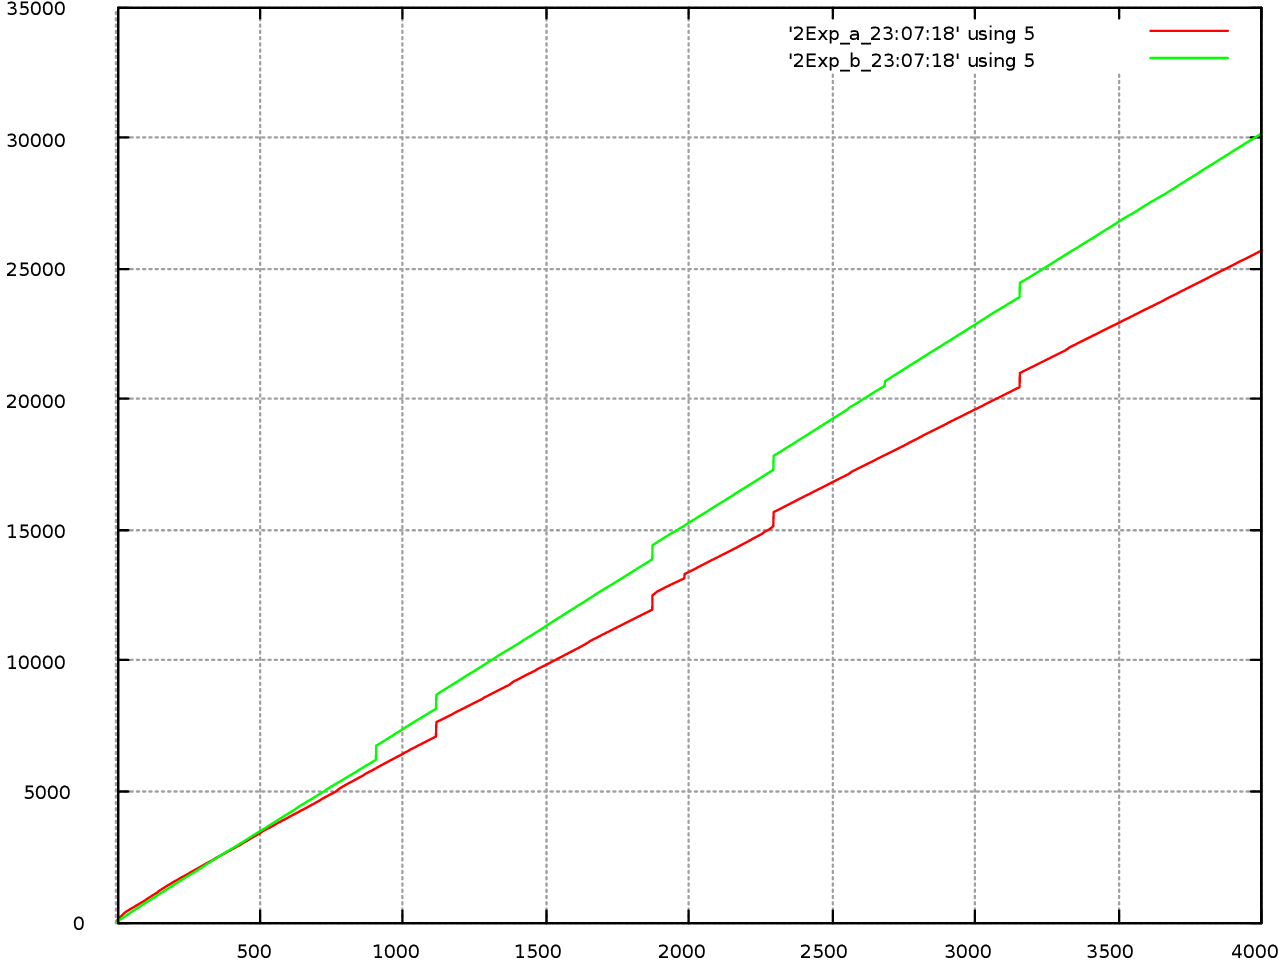
\includegraphics[width=12cm]{img/exec-time} 
\end{figure}

\section{Interim results}

Since the relative error seems to be in control with the improved algorithm for as many as 100 000 rankings we can assume that it would produce good enough rankings for five hours.

The execution time with the current implementation for five hours would then be $5 \times 6 \times 10 205 ms + \frac{100 000}{4000} \times 25 687 = 948 325 ms$

For the improved algorithm, $10 205 ms + \frac{100 000}{4000} \times 30 180 = 764705 ms$.

